\documentclass[margin=0mm]{standalone}
\usepackage{tikz}
\usepackage{pgfplots}
 \pgfplotsset{compat=newest}
\usetikzlibrary{math,matrix,fit,positioning}

\usepackage{tikzorbital}

\newcommand{\benzene}[8]{%
\tikzmath{\x1 = #1; \dx1 = 0.5; \dx2 = 0.9; \ps=0.5;}
\tikzmath{\x2 = \x1 + \dx1 ;}
\tikzmath{\x3 = \x2 + \dx2 ;}
\tikzmath{\x4 = \x3 + \dx1 ;}

\tikzmath{\y1 = #2; \dy = 0.5;}
\tikzmath{\y2 = \y1 + \dy ;}
\tikzmath{\y3 = \y2 + \dy ;}

\orbital[pos = {(\x1,\y2)},scale=#3 * \ps]{pz}
\orbital[pos = {(\x2,\y1)},scale=#4 * \ps]{pz}
\orbital[pos = {(\x3,\y1)},scale=#5 * \ps]{pz}
\orbital[pos = {(\x4,\y2)},scale=#6 * \ps]{pz}
\orbital[pos = {(\x3,\y3)},scale=#7 * \ps]{pz}
\orbital[pos = {(\x2,\y3)},scale=#8 * \ps]{pz}

\draw (\x1,\y2) -- (\x2,\y1) -- (\x3,\y1) -- (\x4,\y2) --(\x3,\y3) 
-- (\x2,\y3) -- (\x1,\y2);
}


\begin{document}

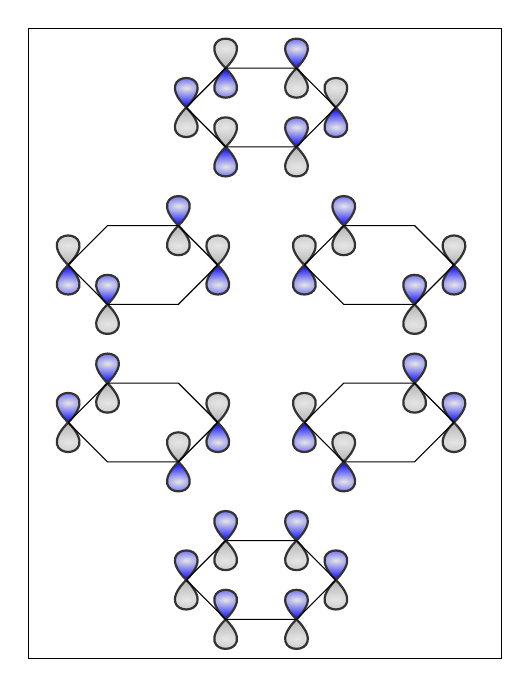
\begin{tikzpicture} 
%\useasboundingbox (0.7,-0.2) rectangle (4,4);
\draw (-2,-0.5) rectangle (4,7.5);

%((1, 1, 1, 1, 1, 1), (1, 0, -1, -1, 0, 1), (-1, -1, 0, 1, 1, 0), (-1, 1, 0, -1, 1, 0), (-1, 0, 1, -1, 0, 1), (-1, 1, -1, 1, -1, 1)) 
\benzene{0}{0}      {1}{1}{1}{1}{1}{1}
\benzene{-1.5}{2} {1}{0}{-1}{-1}{0}{1}
\benzene{1.5}{2}   {-1}{-1}{0}{1}{1}{0}
\benzene{-1.5}{4} {-1}{1}{0}{-1}{1}{0}
\benzene{1.5}{4}  {-1}{0}{1}{-1}{0}{1}
\benzene{0}{6}{1} {-1}{1}{-1}{1}{-1}{1}

\end{tikzpicture}



\end{document}